\newpage
%%%%%%%%%%%%%%%%%%%%%%%%%%%%%%%%%%%%%%%%%%%%%%%%%%%%%%%%%%%%%%%%%%%%%%%%%%%%%%%
\section{Week 8?}
%%%%%%%%%%%%%%%%%%%%%%%%%%%%%%%%%%%%%%%%%%%%%%%%%%%%%%%%%%%%%%%%%%%%%%%%%%%%%%%
\subsection*{Sunday, 06/10/2024}
\begin{itemize}
    \item we might be back (leptos rewrite). notes from testing existing hubble
        node routes with leptos components.
    \item this is not live yet since it has very limited funtionality.
    \item \texttt{fetch_username} checks if \texttt{lead_usernames} already 
        has the \texttt{fid}. if not, it fetches the username and updates the 
        state.
    \item added \texttt{ongoing_requests} to track fetches and avoid multiple 
        requests for the same \texttt{fid}.
    \item Used \texttt{create_effect} to manage side effects, ensuring 
        usernames are fetched only once.
    \item Used \texttt{spawn_local} for async tasks to keep the main thread 
        non-blocking.
    \item \texttt{Signal} and \texttt{set_signal} handle reactive state in the 
        \texttt{Channels} component, making sure the UI updates when data 
        changes.
    \item \texttt{HashSet} tracks \texttt{ongoing_requests}, preventing 
        duplicate fetches and redundant state updates.
    \item The component dynamically displays usernames from the updated state.
    \item asdfasdf
\end{itemize}

\subsection*{Monday, 06/11/2024}
\begin{itemize}
    \item removed the \texttt{lead_username} variable and its assignment using 
        \texttt{unwrap_or_else} from the \texttt{view!} macro.
    \item added closure inside the \texttt{view!} macrothat matches on 
        \texttt{lead_usernames.get().get(<ref>fid)}.
    \item if the lead username is available show it, else show "chill" in div
        where username would be 
    \item closure is defined using \texttt{move ||} to capture the 
        \texttt{lead_usernames} and \texttt{fid} variables.
\end{itemize}

\clearpage
\subsection*{Tuesday, 06/12/2024}
\begin{itemize}
    \item begin rewrite of cast and cast list pages, need to think about using 
        \texttt{create_effect} in the complicated way that i did above.
    \item using this \texttt{create_effect} in the way that i am to sync the
        reactive system is \textit{officially} 
        (Figure~\ref{fig:create_effect_bad}) discouraged since you might shoot
        off your foot with an infinite loop if you don't create something to
        keep track of the ongoing_requests. i liike the chill message though and
        how it could show up at different times for different channels in some
        cases (probably won't be used, but we will see).
    \item i'll do the cast stuff without \texttt{create_effect} to see
        if it's less complicated and achieves virtually the same thing. 

        \begin{figure}[ht]
            \centering
            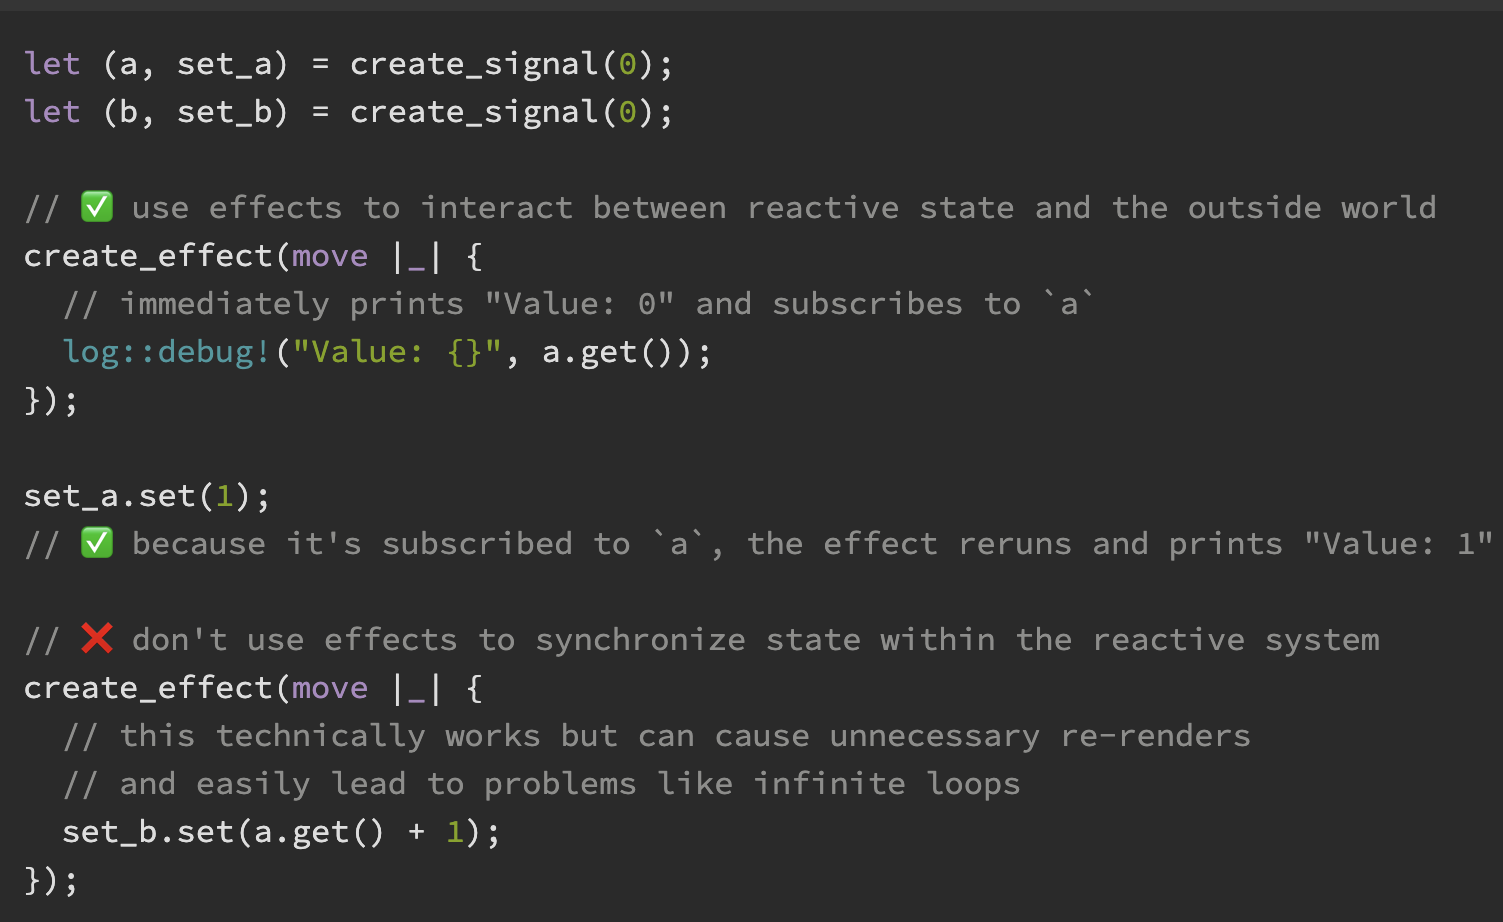
\includegraphics[width=15cm]{create_effect_bad}
            \captionsetup{labelfont=bf, textfont=it}
            \caption{create effect bad}
            \label{fig:create_effect_bad}
        \end{figure}
\end{itemize}
